\documentclass[aspectratio=169,10pt]{beamer}
\usepackage{amssymb,amsmath,amsthm,enumerate}
\usepackage[utf8]{inputenc}
\usepackage{array}
\usepackage[parfill]{parskip}
\usepackage{graphicx}
\usepackage[
bookmarksopen,
bookmarksdepth=2,
breaklinks=true
]{hyperref}
\usepackage{caption}
\usepackage{subcaption}
\usepackage{bm}
\usepackage{amsfonts,amscd}
\usepackage[]{units}
\usepackage{listings}
\usepackage{multicol}
\usepackage{multirow}
\usepackage{tcolorbox}
\usepackage{physics}
\date{26 Ocak 2021}
\logo{
\includegraphics[height=0.9cm]{cf674d69eebd62dcc9bcd14cd04488b9.png}\hspace{20pt}\vspace{0pt}} 
\usetheme{Stanford} 

\def \ai {\item[] \quad \arrowbullet}
\newcommand \si[1]{\item[] \quad \bulletcolor{#1}}
\def \wi {\item[] \quad $\ \phantom{\Rightarrow}\ $}
\def \bi {\begin{itemize}\item}
\def \ei {\end{itemize}}
\def \be {\begin{equation*}}
\def \ee {\end{equation*}}
\def \bie {$\displaystyle{}
\def \eie {{\ }$}}
\def \bsie {\small$\displaystyle{}
\def \esie {{\ }$}\normalsize\selectfont}
\def \bse {\small\begin{equation*}}
\def \ese {\end{equation*}\normalsize}
\def \bfe {\footnotesize\begin{equation*}}
\def \efe {\end{equation*}\normalsize}
\renewcommand \le[1] {\\ \medskip \lefteqn{\hspace{1cm}#1} \medskip}
\def \bex {\begin{example}}
\def \eex {\end{example}}
\def \bfig {\begin{figure}}
\def \efig {\end{figure}}
\def \btheo {\begin{theorem}}
\def \etheo {\end{theorem}}
\def \bc {\begin{columns}}
\def \ec {\end{columns}}
\def \btab {\begin{tabbing}}
\def \etab {\end{tabbing}\svneg\svneg}
\newcommand \col[1]{\column{#1\linewidth}}
\def\vneg  {\vspace{-5mm}}
\def\lvneg {\vspace{-10mm}}
\def\svneg {\vspace{-2mm}}
\def\tvneg {\vspace{-1mm}}
\def\vpos  {\vspace{5mm}}
\def\lvpos {\vspace{5mm}}
\def\svpos {\vspace{2mm}}
\def\tvpos {\vspace{1mm}}
\def\hneg  {\hspace{-5mm}}
\def\lhneg {\hspace{-10mm}}
\def\shneg {\hspace{-2mm}}
\def\thneg {\hspace{-1mm}}
\def\hpos  {\hspace{5mm}}
\def\lhpos {\hspace{10mm}}
\def\shpos {\hspace{2mm}}



\ 

\title{Dirac Denkleminin İncelenmesi}

\begin{document}

\author[Halil Kolatan]{
	\begin{tabular}{c} 
	\huge
	Halil Kolatan
\end{tabular}
\vspace{-3ex}}

\institute{


\  

	\vskip 5pt
	\begin{figure}
		\centering
		\begin{subfigure}[t]{0.2\textwidth}
			\centering
			
\includegraphics[height=0.7in]{cf674d69eebd62dcc9bcd14cd04488b9.png}
		\end{subfigure}%
		~ 
		\begin{subfigure}[t]{0.2\textwidth}
			\centering
			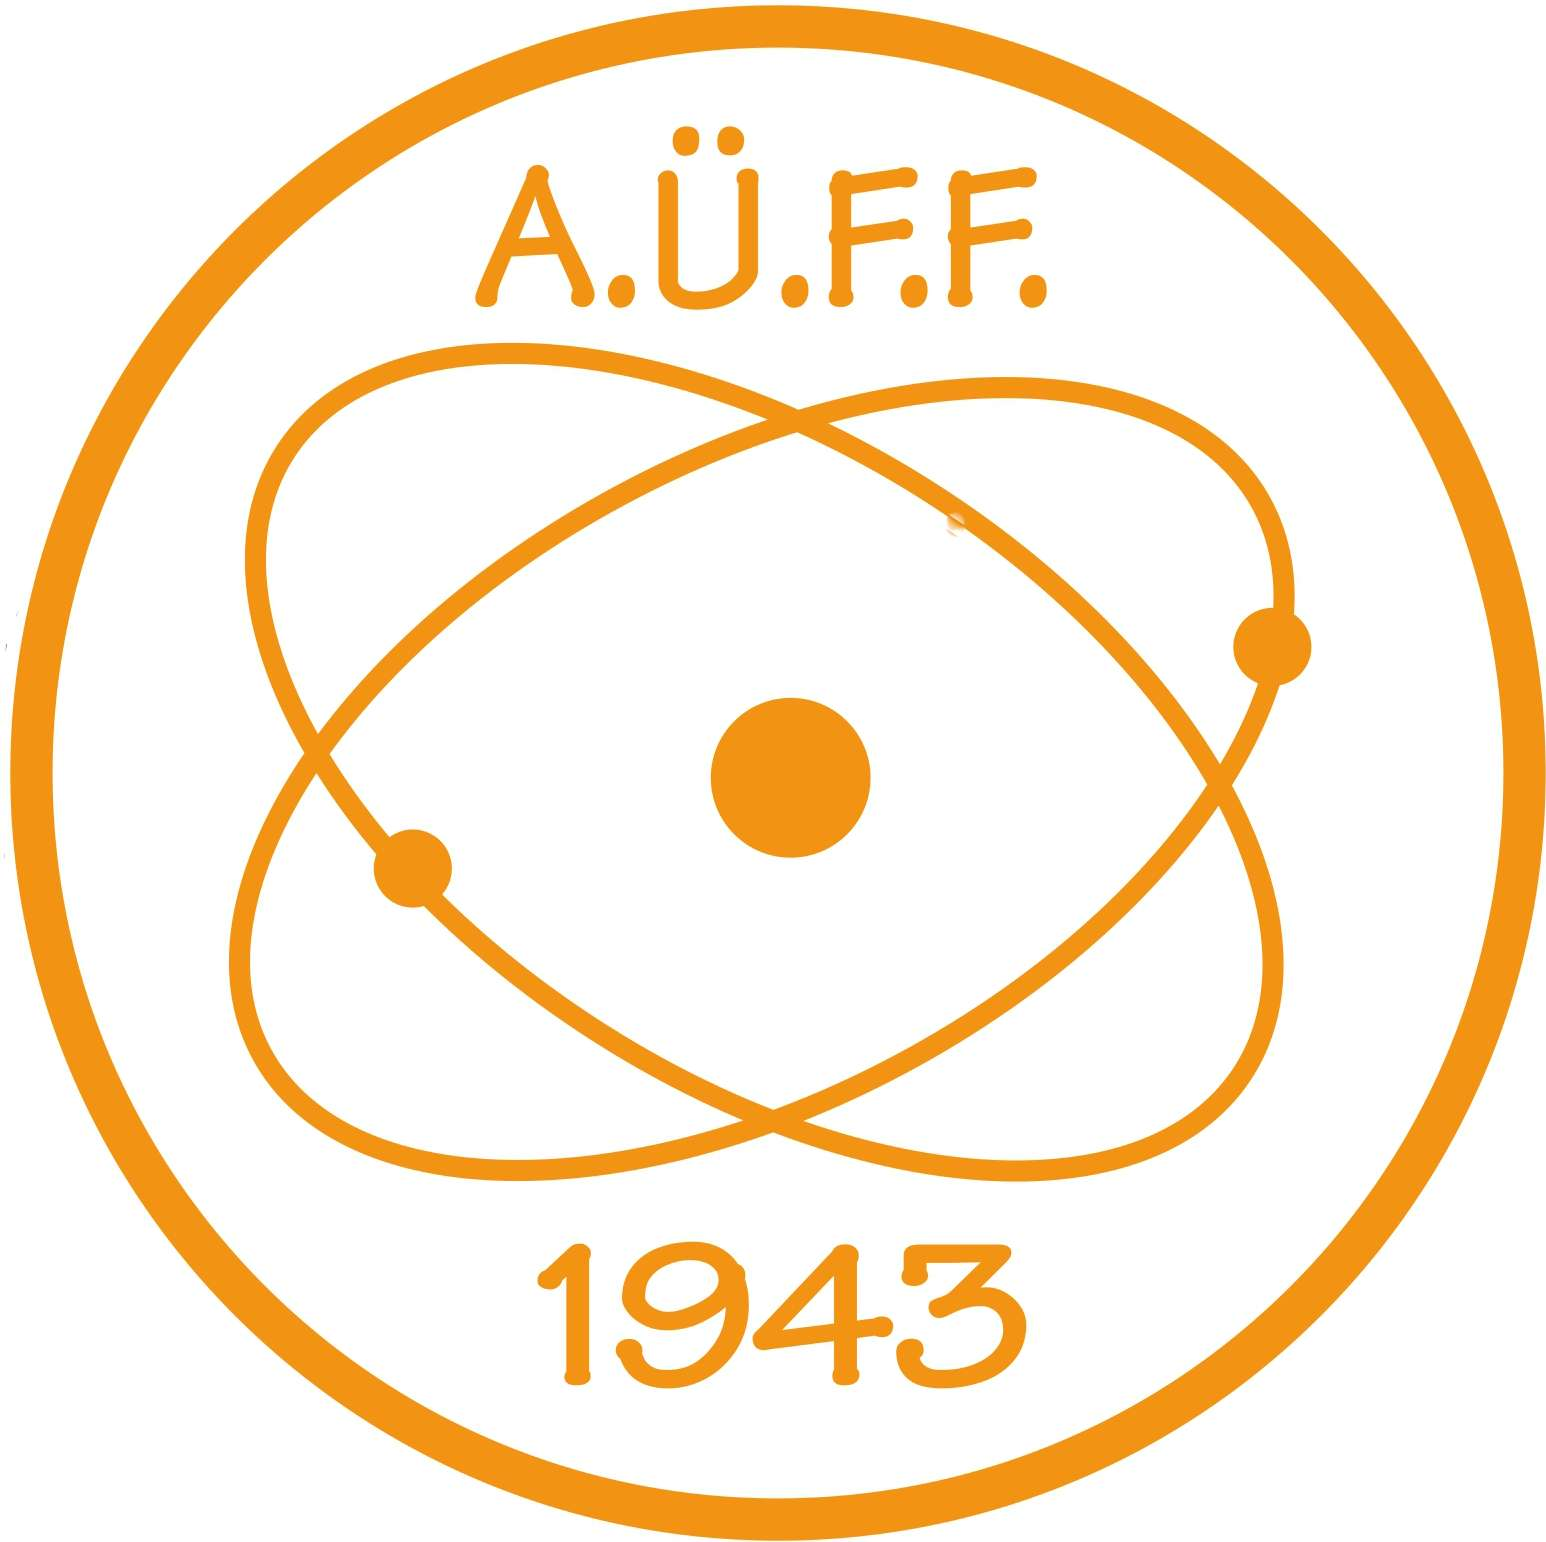
\includegraphics[height=0.7in]{Ankara-Üniversitesi-Fen-Fakültesi.png}
		\end{subfigure}
	\end{figure}
	
	\ 
	
	
	\vskip 5pt\\
	\Large
	Fiz0423 - Özel Görelilik Teorisi \\
	\ 
	Ankara Üniversitesi\\
	\vskip 3pt
	
}

\setbeamertemplate{itemize items}[default]
\setbeamertemplate{itemize subitem}[circle]
 
\begin{frame}[plain]
\titlepage \end{frame}

\begin{frame}
	\frametitle{İçerik} % Table of contents slide, comment this block out to remove it
	\tableofcontents % Throughout your presentation, if you choose to use \section{} and \subsection{} commands, these will automatically be printed on this slide as an overview of your presentation
\end{frame}

	
    \section{Paul Adrien Maurice Dirac}
    
    \begin{frame}[allowframebreaks]
\frametitle{Paul Adrien Maurice Dirac}

\begin{columns}

\column{0.5\textwidth}
 Elektronun rölativistik dalga denklemini, anti-parçacıklar fikrini, kuantum elektrodinamiğinin basit ancak önemli yorumunu, manyetik monopoller kuramını açıklığa kavuşturarak kuantum mekaniğinin gelişmesine önemli katkılar sağlayan ünlü bilim insanı Paul Dirac, 8 Ağustos 1902'de Bristol'da doğmuştur. Dirac 1921 yılında Bristol Üniversitesi elektrik mühendisliği bölümünden mezun olmuştur. 1921'de üniversiteyi bitiren Dirac, teorik fizik çalışmalarına başlamadan önce iki yıl daha matematik okumuştur. Yüksek lisans için burslu olarak Cambridge Üniversitesine gitmiştir. Cambridge'de danışmanı dönemin ünlü fizikçisi Rutherford'un damadı Ralph Fowler olmuştur [1].

\column{0.5\textwidth}
\centering
 \begin{figure}
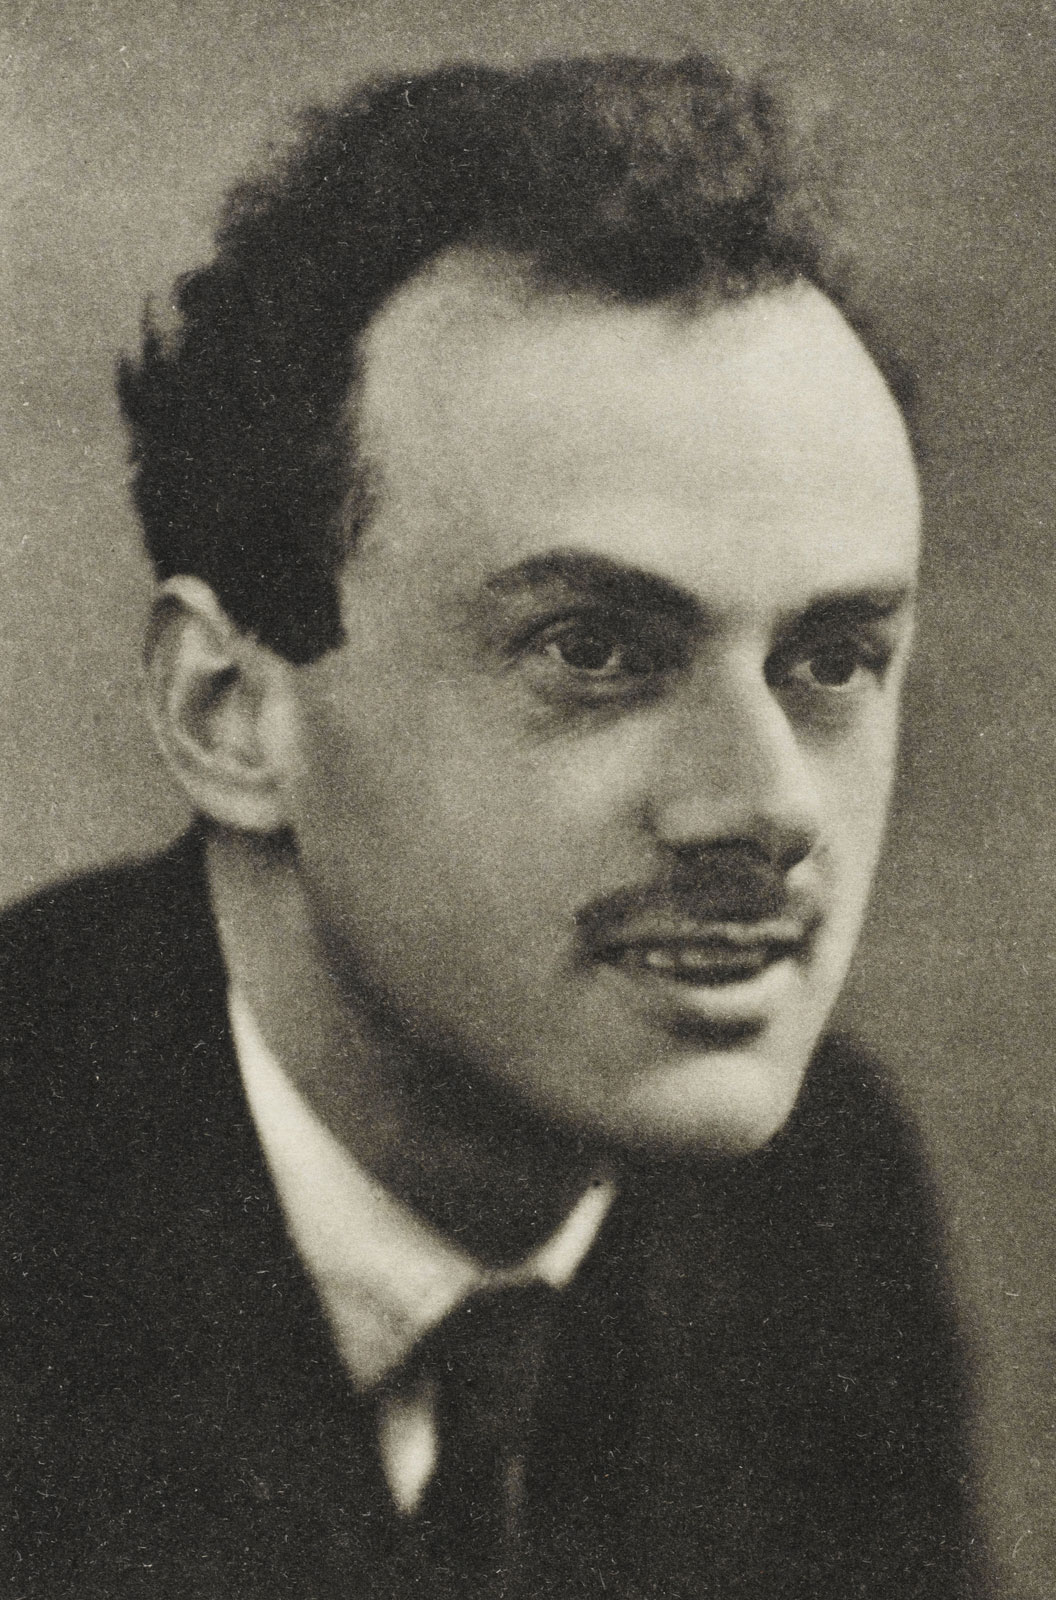
\includegraphics[width=3.5cm]{PAM-Dirac.jpg}
\caption*{Paul Adrien Maurice Dirac [2].}
	\end{figure}

\end{columns}

\end{frame}

\begin{frame}[allowframebreaks]
\frametitle{Paul Adrien Maurice Dirac}


 Dirac, yeteneği ile başta Fowler'in olmak üzere birçok bilim insanının dikkatini üzerine çekmeyi başarmıştır. Çok geçmeden istatiksel mekanik ve kuantum mekaniği üzerine yapmış olduğu araştırmaları yayımlamıştır. Fowler'in kuantum mekaniği ile ilgili makalesini inceleyen Dirac, makalenin devrim niteliğindeki önemini kavramış ve çalışmalara başlamıştır. 1926 yıllı doktora tezinin temelini de oluşturan makaleleri kuantum mekaniği üzerine yapılan çalışmalara paralellik göstermektedir. Dirac, klasik mekanikte kullanılan Poisson parantezleri metoduyla, kuantum mekaniği için W. Heisenberg tarafından yeni önerilen matris arasındaki benzerliklerin farkına varmış ve bu gözlemleriyle 1926 yılındaki yazdığı makalesiyle Cambridge'den Ph. D. unvanını almıştır. Birkaç yıl sonra Dirac, farklı boyutlar kazandırdığı kuantum fiziğinin lideri durumuna gelmiştir. En yaratıcı dönemiyse 1925-1933 yılları arasında olmuştur. Bu dönemde günümüz kuantum mekaniğinde temel önemi olan yepyeni kuramlar geliştirmiştir. Fermi-Dirac istatistiği olarak bilinen kuramı 1927 yılında bağımsız olarak geliştirmiş ardından kuantum elektrodinamiği konusunda öncülük eden "\textit{Işınım Yayımı ve Soğurulmasının Kuantum Kuramı"} adlı makalesini yazmıştır [1].



\end{frame}

\begin{frame}[allowframebreaks]
\frametitle{Paul Adrien Maurice Dirac}


Sonraki yıl elektronlar için relativistik dalga denklemini geliştirmiş bu yöntemle daha önce yalnızca bir doğa olayı olarak bilinen spin ve manyetik moment kavramlarını açıklamıştır. Nitekim bu çalışmalar 1934 yılında Dirac'ın karşı-elektron ve genel olarak anti-parçacıkların varlığını ortaya koymasını sağlayan fikirlerinin temelini oluşturacak derecede büyük önem taşımaktadır [1]. 

1930 yılında henüz yirmi sekiz yaşındayken Royal Society'e seçilen Dirac ertesi yıl Lucas kürsüsünde matematik profesörlüğüne atanmıştır. 1933 yılında Dirac ve Schrödinger "\textit{atom kuramının sonuç getiren yeni formlarını keşfetmelerinden dolayı"} Nobel Fizik Ödülü'nü paylaşırlar. Yedinci Solvay Konferası'nda \textit{Atom Çekirdeğinin Yapısı ve Özellikleri} başlıklı bir konuşma yapmıştır [1].

Dirac'a göre fiziğin amacı dünyanın özelliklerini ortaya koymak değil, yalnızca deneysel sonuçları hesaplama yöntemlerini sağlayacak somut sistemler oluşturmaktır. Kuantum mekaniğinin yorumlanması gibi felsefi önemi olan daha kapsamlı sorular ilgisini hiçbir zaman çekmemiştir [1].

Dirac, 20 Ekim 1984 tarihinde hayatını kaybetmiştir.


\end{frame}
	
	\section{Dirac Denkleminin Tarihsel Gelişimi}
	
	
	\begin{frame}[allowframebreaks]
\frametitle{Dirac Denkleminin Tarihsel Gelişimi}

Steven Weinberg, \textit{Four golden lessons} adlı makalesinde genç araştırmacılara öğütler verirken, özetle çalışmaların doğru problemler üzerine yapılmasının gerekliliğini
ve yaratıcı çalışmalar üretmek için gereken zamanın çok büyük bir kısmının
yaratıcı olmayan çalışmalara harcanması gerektiğini söyler. Bilimsel çalışmalar
yapılırken karşılacak bu gibi durumlarla başa çıkabilmek için bilim tarihi
öğrenmenin, en azından uğraşılan bilim dalının tarihini öğrenmenin çok önemli
olduğunu vurgular. Bilim insanlarının zamanımızın veya öncesinin filozoflarının
öne sürdüğü aşırı basitleştirilmiş modellere inanmalarının yaptıkları işleri
zorlaştırdığını, zorlaştıracağını söyledikten sonra buna en iyi ilacın bilim tarihi
bilgisinin olduğunu söyler. Bilimsel çalısmalar yapmanın toplum tarafından
anlaşılamaması, çalışmayı yapanların yaptıkları işten tatmin olma hissi
duymadıklarından, çalışmanın değerinin olmadığını düşünmelerine neden
olduğunu belirtip, bilim tarihi bilmek yapılan çalışmayı bu tarih içinde bir yere
yerleştirmeyi sağladığından, çalışmayı sizin için daha değerli yapacağını vurgular [3,4].



\end{frame}
	
	
	
\begin{frame}[allowframebreaks]
\frametitle{Dirac Denkleminin Tarihsel Gelişimi}

Schrödinger, de Broglie’nin dalga-parçacık hipotezini gördüğünde bu durumun ancak rölativistik çerçevede bir anlamının olduğunu bildiğinden Hidrojen atomunu rölativistik olarak ele almıştır. Fakat bu rölativistik teoriyi tamsayı yerine yarım tamsayı kuantum sayılarına sahip olduğundan bırakmıştır. Rölativistik olmayan, yaklaşık çözümler üreten başka bir teori geliştirmeye
başlamıştır. Deneysel sonuçlara uygun sonuçlar veren teorilerde ısrar eden bir kişilige sahip olduğundan, Schrödinger’in rölativistik teoriyi bir kenara bırakması çok doğal bir davranış olarak karşılanmıştır. Schrödinger yaptığı çalışmaları anlatmak üzere gittiği Münih üniversitesinde sorulan sorular üzerine rölativistik bir dalga denklemi yazmıştır. Yazılan bu
denklemin sıfır potansiyeller için yazılan çeşitli formları birçok isme ait olarak
gösterilmiştir. Bu karmaşıklığın nedeni Schrödinger’den sonra yapılan çalışmaların hemen hepsinin Schrödinger’in bu seminerde yazdığı denklemden çıkmasıyla açıklanabilir . Bu denklemin en saf hali Pauli’nin Jordan’a yazdığı bir mektupta matris mekaniği ve Schrödinger dalga denkleminin
denkliğini gösterirken ortaya çıkmıştır [4].



\end{frame}


\begin{frame}[allowframebreaks]
\frametitle{Dirac Denkleminin Tarihsel Gelişimi}

Klein 1925 nisanında yaptığı bir çalışmada daha önce Kaluza’nın öne sürdüğü elektromagnetik teori ve gravitasyon alanı arasındaki ilişki ile kuantum mekaniği problemlerinde Schrödinger ve de Broglie yöntemlerinin sunduğu çözümler arasında basit bir ilişki bulduğunu belirtmiştir. 5 boyutlu uzayda yazılan, genel rölativite teorisi sembollerinin genelleştirilmesini içeren diferansiyel denklemden, minimum vektör potansiyel için ikinci derece dalga denklemi ve çözümü
yazılmıştır [4].

Schrödinger denkleminin genelleştirilmesi için Fock ve Gordon çalışmalar yapmıştır. 1926’da Gordon "Schrödinger teorisine göre Compton olayı" başlıklı yayınında, tamamen rölativistik bir formda Schrödinger denkleminin en uygun matematiksel temsilini vermiştir. Daha sonra bu denklemin nasıl bir atomdan yayınlanan radyasyonu elde etmek için kullanılacağını gösterdi. Bu şekilde
çalışarak Compton olayını tanımlayan rölativistik dalga denklemini ve bu denklemden Compton radyasyonunun gücünü elde etti [4].



\end{frame}

\begin{frame}[allowframebreaks]
\frametitle{Dirac Denkleminin Tarihsel Gelişimi}

Dirac’ın Kopenhag ziyaretinde, Bohr, Dirac’a ne üzerine çalıştığını sorduğunda, Dirac elektronun tatmin edici bir rölativistik teorisini elde etmeye çalıştığını söyler. Bohr buna karşılık bu işin zaten Klein ve Gordon tarafından yapılmış oldugunu söyler. Bu yanıt Dirac’ı oldukça rahatsız eder, Bohr’u Klein’ın verdiği çözümden oldukça memnun olarak görür. Fakat Dirac Klein-Gordon denkleminde ortaya çıkan negatif olasılık değerlerinden rahatsız olduğundan, negatif olasılıkları ortadan kaldıracak ve sadece pozitif olasılıklara sahip bir teori için çalışmalarına devam etmiştir. Dirac daha önce matris mekaniği ve dalga mekaniği arasındaki özdeşliği gösterirken ortaya koyduğu dönüşüm teorisinin genel formunun çok güçlü bir araç olduğunu ve rölativistik
uygulamalarda kullanılabileceğini düşündü. Bunun yapılabilmesi için Schrödinger denklemi gibi zamanda lineer olan bir dalga denklemine gereksinim duydu [4].



\end{frame}

\begin{frame}[allowframebreaks]
\frametitle{Dirac Denkleminin Tarihsel Gelişimi}

1928’de Dirac elektron için yazdığı rölativistik dalga denklemini yayımladı. Bu denklem pozitif enerji değerleri yanında negatif enerji değerlerinde çözümleri de içeriyordu. Bu durumun açıklanması bir çok zorluk çıkardı. Dirac elektron denizinde boşluğun pozitif yüklü bir parçacık gibi görüneceğini öne sürerek negatif enerji değerlerinin o zamanlar bilinen tek pozitif yüklü parçacık olan protona ait olması gerektiğini söyledi. Fakat elektron ve proton kütleleri
arasındaki farkın büyüklüğü bu söylemini bırakmasına neden oldu. Daha sonra bu negatif enerji değerlerinin kütlesi elektron kütlesine eşit ve yükü elektron yükünün zıddı olan bir parçacığı temsil ettiğini istemeyerek de olsa söylemek zorunda kaldı. Bu parçacığın ismini anti-elektron olarak koydu [4].



\end{frame}

\begin{frame}[allowframebreaks]
\frametitle{Dirac Denkleminin Tarihsel Gelişimi}

\begin{columns}


	\column{0.5\textwidth}

1932’de Anderson kozmik ışımalarda bu parçacığı gözledi ve ismini değiştirerek pozitron olarak adlandırdı. Dirac denkleminin çözümlerinin bu şekilde bir anti-parçacık betimlemesi de içermesi, temel parçacık kavramını tümden degiştirdi. Dirac denkleminin yazılmasından önce Pauli, spin operatörünün baz vektörleri olarak Pauli spin matrislerini yazmıştı. Bu matrisler Dirac denkleminde parçacık ve anti-parçacık için ayrı ayrı ortaya çıktıklarından, çözüm toplamda 4 bileşene sahip olan genelde spinör denen bir dalga fonksiyonu olur [4].

\column{0.5\textwidth}

\centering
 \begin{figure}
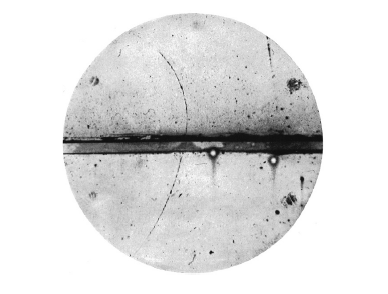
\includegraphics[width=5cm]{pozitron..PNG}
\caption*{Anderson tarafından bir Wilson bulut odasında gözlemlenen ilk pozitron izlerinden biri. Anderson 1933. American Physical Society'den [7].}
	\end{figure}
	


\end{columns}
\end{frame}


\begin{frame}[allowframebreaks]
\frametitle{Dirac Denkleminin Tarihsel Gelişimi}

Dirac’ın 1926’da yazdığı kuantum mekaniksel dönüşüm teorisiyle birlikte rölativistik elektron teorisinden yola çıkılarak kuantum alan teorisinin ilk temelleri atılmıştır. Bu teori ile elektronun bir foton ile etkileşmesi tanımlanmaya çalışılmıştır. Tamamen rölativistik bir çerçeveden elektron-ışık etkileşmesinin de tanımını veren kuantum elektrodinamiği teorisi, Lorentz ve Abraham tarafından kurulmak istenen elektronun rölativistik teorisidir. Bu teori ile kuantum mekaniğinin genel yapısı anlamlı bir şekilde elektronun formundan bağımsız olarak, rölativistik elektromagnetik teori ile birleştirilmiştir [4].



\end{frame}
	
	
	\section{Dirac Denkleminin İncelenmesi}
	\begin{frame}[allowframebreaks]
\frametitle{Dirac Denkleminin İncelenmesi}

Rölativistik dalga denklemi oluşturabilmek için doğru bir rölativistik enerji-momentum ilişkisi yazılmalıdır. Bunun için öncelikle uzay ve zaman bileşenlerini içeren enerji - momentum 4-vektörü tanımlanır [5]:
\begin{align}
    p^{\mu} = \big( \dfrac{E}{c},\Vec{p} \big), \quad p_{\mu} = \big( \dfrac{E}{c},-\Vec{p} \big)
\end{align}
\begin{align}
    p^{2} = p^{\mu}p_{\mu} = \dfrac{E^{2}}{c^{2}} - \Vec{p} \cdot \Vec{p} = m^{2} c^{2}
\end{align}
Denklem (1) yeniden yazılarak enerjinin karesi ifadesi elde edilir.
\begin{align}
    E^{2} = p^{2} + m^{2}
\end{align}
\end{frame}



	\begin{frame}[allowframebreaks]
\frametitle{Dirac Denkleminin İncelenmesi}

Kuantum mekaniğinin temel varsayımlarından biri, fiziksel gözlenebilirlere bir işlemcinin karşılık geldiğidir. Bu işlemciler çizgisel ve hermitseldir. Enerji ve momentumun işlemci karşılıkları
\begin{align}
    p^{\mu} = -i \hbar \Vec{\nabla}, \quad E=i \hbar \dfrac{\partial}{\partial t}
\end{align}
şeklindedir. Kuantum mekaniğinde bir sistem belli bir t anında, türevlenebilir ve sürekli $ \psi (\Vec{r},t) $ dalga fonksiyonu ile tanımlanır. Klasik toplam enerji ifadesinde enerji
ve momentum yerine işlemci karşılıkları yazılıp, bu işlemciler dalga fonksiyonu üzerine etkirse
Schrödinger denklemi elde edilir.
\begin{align}
    - \dfrac{\hbar^{2}}{2m} \Vec{\nabla}^{2} \psi + V \psi = i \hbar \dfrac{\partial \psi}{\partial t}
\end{align}
\end{frame}

	\begin{frame}[allowframebreaks]
\frametitle{Dirac Denkleminin İncelenmesi}

Göreli enerji-momentum-kütle bağıntısı ile başlayarak Klein-Gordon (KG) denklemi elde edilebilir.
\begin{align}
    p^{2} = p^{\mu}p_{\mu} = \dfrac{E^{2}}{c^{2}} - \Vec{p} \cdot \Vec{p} = m^{2} c^{2}
\end{align}
\begin{align}
    p^{\mu} \rightarrow -i \hbar \partial_{u}
\end{align}
\begin{align}
\Vec{p} \rightarrow -i \hbar \Vec{\nabla}, \quad E \rightarrow i \hbar \dfrac{\partial}{\partial t}
\end{align}
Denklem (6) böylece şunu verir,
\begin{align}
    \bigg( \dfrac{1}{c^{2}}\dfrac{\partial^{2}}{\partial t ^{2}} - \nabla^{2} \bigg) \phi + \dfrac{m{2}c^{2}}{\hbar^{2}} \phi = 0
\end{align}



\end{frame}

	\begin{frame}[allowframebreaks]
\frametitle{Dirac Denkleminin İncelenmesi}


Klein-Gordon denklemi (9) elde edilmiş olur. Denklemde görülen $\phi(x,t) $ skaler dalga fonksiyonudur. Klein-Gordon denklemi spin-0 bozonları tanımlamak için uygundur. Bu denklem enerji eşitliği için yeniden yazıldığında enerjinin negatif değerli çözümünün ihmal edilemeyeceği görülür. \\ 
Klein-Gordon denklemi hem zamana hem de uzaysal koordinatlara göre ikinci mertebe türevleri içermektedir. Göreli enerji-momentum bağıntısından hareketle elde edilen Klein-Gordon denkleminin tek parçacık göreli dalga denklemi olarak yorumlanmasında; \\

\

i)   negatif enerjili çözümlerin bulunuşu, \\

\

ii) olasılık yoğunluğunun pozitif tanımlı olmayışı gibi iki zorluk ortaya çıkmıştır.



\end{frame}

	\begin{frame}[allowframebreaks]
\frametitle{Dirac Denkleminin İncelenmesi}

Dirac 1928 yılında enerji ve momentumun lineer olarak ilişkili olduğu bir denklem yazar. Göreli kovaryantlığın (tüm eylemsiz gözlem çerçevelerinde denklemin formunun aynı olmasının) sağlanması için bu denklem, hem $\partial / \partial t$ terimine hem $ \Vec{\nabla}$ terimine göre çizgisel olmalıdır [6]. Serbest parçacık için Dirac denklemi;

\begin{align}
    \hat{E} \psi = H\psi
\end{align}
\begin{align}
    i \hbar \dfrac{\partial \psi}{\partial t} = ( c \Vec{\alpha} \cdot \Vec{p} + \beta mc^{2} ) \psi
\end{align}
\begin{align}
    i \hbar  \dfrac{\partial \psi}{\partial t} = \Bigg[  \dfrac{\hbar c}{i} \sum_{i} \alpha_{i} \dfrac{\partial}{\partial x^{i}}  + \beta mc^{2} \Bigg] \psi
\end{align}



\end{frame}

	\begin{frame}[allowframebreaks]
\frametitle{Dirac Denkleminin İncelenmesi}

Bileşenler cinsinden;

\begin{align}
    i \hbar \dfrac{\partial \psi_{\lambda}}{\partial t} = \dfrac{\hbar c }{i} \sum_{\delta = 1}^{N} ( \alpha_{1} \dfrac{\partial}{\partial x^{1}} + \alpha_{2} \dfrac{\partial}{\partial x^{2}}+ \alpha_{3} \dfrac{\partial}{\partial x^{3}}  )_{\lambda \delta} \psi_{\delta} + mc^{2} \sum_{\delta = 1}^{N} \beta_{\lambda \delta} \psi_{\delta}
\end{align}
elde edilir. İstenilen denkleme ulaşmak için $\alpha$ ve $\beta$ katsayılarının belirlenmesi gerekir. Uzaysal dönmeler altında denklem (12)’ nin değişmez kalabilmesi için $\alpha_{i}$'ler $(i=1,2,3)$ sayı olmamalıdırlar. Dalga fonksiyonu $\psi$, $N \times 1 $' lik sütun matris olmak üzere, $\alpha_{i}$ 'ler $N \times N$ 'lik matrislerdir.



\end{frame}


	\begin{frame}[allowframebreaks]
\frametitle{Dirac Denkleminin İncelenmesi}

Bunları bulabilmek için öncelikle göreli bir dalga denklemi kurmak için gerekli özellikleri özetleyelim: \\

\

1) E ve $\Vec{p}$ arasında göreli bir ilişki $\rightarrow   E^{2} = \Vec{p}^{2}c^{2} + m^{2} c^{4} $; \\

\

2) Olasılık yoğunluğu durumu için $\rho \geq 0$; \\

\ 

3) Lorentz dönüşümleri altında kovaryantlık (form değişmezliği).



\end{frame}

	\begin{frame}[allowframebreaks]
\frametitle{Dirac Denkleminin İncelenmesi}

İlk özelliğin sağlanabilmesi için, dalga fonksiyonunun her bir bileşeninin ($\psi_{\lambda}$'ların) daha önce denklem (9) ile verilen Klein-Gordon denklemini sağladığını düşünüyoruz.
\begin{align}
    -\hbar^{2} \dfrac{\partial^{2} \psi_{\lambda} }{\partial t^{2}} = \bigg[ -\hbar^{2} c^{2} \Vec{\nabla}^{2}  + m^{2}c^{4} \bigg]\psi_{\lambda}
\end{align}
Bundan sonra amacımız Dirac denklemini Klein-Gordon denkleminin formuna benzetebilmektir. Bunun için denklem (12) ile yazılan Dirac denkleminin zamana göre türevini alalım ve $i \hbar$ ile çarpalım.
\begin{align}
    -\hbar^{2} \dfrac{\partial^{2} \psi}{\partial t^{2}} = \bigg[  \dfrac{\hbar c}{i} \sum_{i=1}^{3} \hat{\alpha}_{i} \dfrac{\partial}{\partial x^{i}} + \beta mc^{2} \bigg] i \hbar \dfrac{\partial_{\psi}}{\partial t}
\end{align}

\end{frame}


	\begin{frame}[allowframebreaks]
\frametitle{Dirac Denkleminin İncelenmesi}
Denklem (15), denklem (12)'de yerine konulup düzenleme yapılırsa;
	
	\begin{align}
	    -\hbar^{2} \dfrac{\partial^{2} \psi}{\partial t^{2}} = \bigg[  \dfrac{\hbar c}{i} \sum_{i=1}^{3} \hat{\alpha}_{i} \dfrac{\partial}{\partial x^{i}} + \beta mc^{2} \bigg] \bigg[  \dfrac{\hbar c}{i} \sum_{j=1}^{3} \hat{\alpha}_{j} \dfrac{\partial}{\partial x^{j}} + \beta mc^{2} \bigg] \psi
	\end{align}
	\begin{align}
	    -\hbar^{2} \dfrac{\partial^{2} \psi}{\partial t^{2}} = -\hbar^{2} c^{2} \sum_{i,j=1}^{3} \dfrac{\alpha_{i}\alpha_{j} + \alpha_{j}\alpha_{i}}{2} \dfrac{\partial^{2} \psi}{\partial x^{i} \partial x^{j}} + \dfrac{\hbar m c^{3}}{i} \sum_{i=1}^{3} (\alpha_{i} \beta + \beta \alpha_{i}) \dfrac{\partial \psi}{\partial x^{i}} + m^{2} c^{4} \beta^{2} \psi
	\end{align}
\end{frame}

	\begin{frame}[allowframebreaks]
\frametitle{Dirac Denkleminin İncelenmesi}
Denklem (14) ve (17) karşılaştırılırsa $\alpha$ ve $ \beta$ matrisleri için şu koşullar elde edilir: \\
\begin{align}
 \hat{\alpha}_{i} \hat{\alpha}_{j} + \hat{\alpha}_{j}\hat{\alpha}_{i} = 2 \delta_{ij} 1 \rightarrow \{ \alpha_{i} ,\alpha_{j} \} = 0, i \neq j
\end{align}
\begin{align}
 \hat{\alpha}_{i} \hat{\beta} + \hat{\beta}\hat{\alpha}_{i} = 0 \rightarrow \{ \alpha_{i} ,\beta \} = 0
\end{align}
\begin{align}
 \hat{\alpha}_{i}^{2} = \hat{\beta}^{2}  = 1
\end{align}
\end{frame}

	\begin{frame}[allowframebreaks]
	\frametitle{Dirac Denkleminin İncelenmesi}
$\hat{H}$ serbest Dirac hamiltonyeni hermitsel olduğundan $\alpha$ ve $\beta$ matrisleri de hermitseldir.
\begin{align}
    \hat{\alpha_{i}}^{\dag} = \hat{\alpha}_{i}, \quad  \hat{\beta}^{\dag} = \hat{\beta}
\end{align}
$\alpha$ ve $\beta$ matrisleri hermitsel olduğundan öz değerleri reeldir. $\hat{\alpha}_{i}^{2} = \hat{\beta}^{2}  = 1$ koşulundan dolayı özdeğerler $\pm 1$ olabilir. $\alpha$ ve $\beta$ matrislerinin izleri de sıfırdır.
\begin{align}
    ( \hat{\alpha}_{i}\hat{\beta} + \hat{\beta}\hat{\alpha}_{i}=0)\beta
\end{align}
\begin{align}
    \alpha_{i} \beta^{2} = - \beta \alpha_{i} \beta
\end{align}
\begin{align}
    Tr(\alpha_{i}) = -Tr(\beta \alpha_{i}) = -Tr(\beta^{2}\alpha_{i}) = -Tr(\alpha_{i})
\end{align}
\begin{align}
    Tr(\alpha_{i}) = 0 
\end{align}
\begin{align}
    Tr(\beta) = 0 
\end{align}
\end{frame}

	\begin{frame}[allowframebreaks]
	\frametitle{Dirac Denkleminin İncelenmesi}
Denklem (25) ve (26)’dan görüldüğü gibi bu matrislerin izleri sıfırdır. Bu matrislerin
özdeğerlerinin alabileceği değerler $\pm 1$ ve izleri de sıfır olduğu için boyutlarının çift olması gerekir. Bu nedenle N’ nin en küçük değeri 4 olmalıdır. (N=2 Pauli spin matrislerine karşılık gelir). Bir tanımlama ile;

\begin{align}
    \gamma^{0} \equiv \beta \textrm{ ve } \gamma^{i} = \beta \alpha^{i}
\end{align}

istenilen denkleme ulaşılabilinir. $\gamma^{\mu}=(\beta, \beta \Vec{\alpha})$ şeklinde bir tanım yapılır. $\gamma$- matrisleri şu koşulları sağlarlar:

\begin{align}
    (\gamma^{0})^{2} =1, (\gamma^{i})^{2} = -1, \gamma^{\mu} \gamma^{v}   + \gamma^{v}  \gamma^{\mu}  = 0 \quad (\mu \neq v \textrm{ için})
\end{align}

$\gamma$ matrisleri 4x4’lük üniter matrislerdir. Bu matrislerin seçimi tek değildir, farklı temsillerde farklı seçilebilirler.

\end{frame}


	\begin{frame}[allowframebreaks]
	\frametitle{Dirac Denkleminin İncelenmesi}
	Böylece, Dirac denkleminin
	
\begin{align}
	i \hbar \dfrac{\partial \psi }{ \partial t} = H \psi = -i \hbar c \sum_{i}^{} a_{i} \dfrac{\partial \psi}{\partial x_{i}} + \beta m c^{2} \psi
\end{align}
dört boyutlu matris denklemi olduğu yorumuna ulaşıyoruz. Burada $ \psi $, dört boyutlu dalga fonksiyonudur. Dirac spinörü olarak adlandırılır.

\begin{align}
\psi (\textbf{r} , t) = 
	\begin{pmatrix}
	\psi_{1} (\textbf{r} , t) \\  \psi_{2} (\textbf{r} , t)  \\  \psi_{3} (\textbf{r} , t)  \\  \psi_{4} (\textbf{r} , t) 
\end{pmatrix},
\end{align}

\end{frame}

	\begin{frame}[allowframebreaks]
	\frametitle{Dirac Denkleminin İncelenmesi}
	Düzlem dalga çözümleri,

\begin{align}
	\psi (\textbf{r} , t) = u (\textbf{p}) e^{i (\textbf{p} \cdot 	\textbf{r} - Et / \hbar ) },
\end{align}

formunu alır. Burada u(\textbf{p}), aynı zamanda özdeğer denklemini sağlayan dört bileşenli bir spinördür

\begin{align}
	H_{ \textbf{p}} u (\textbf{p}) \equiv (c \alpha \cdot \textbf{p} + \beta mc^{2})u (\textbf{p}) = Eu (\textbf{p}),
\end{align}
(1.10) denkleminde (1.11) yerleştirilmesiyle bulunur. Bu denklemin dört çözümü vardır. Bunlardan ikisi 1/2-spinli parçacıkların iki olası spin durumunu karşılayan $ E = +E_{p} $ (sırasıyla "spin yukarı" ve "spin aşağı" olarak adlandırılır) enerjili çözümler, diğer ikisi de $ E = -E_{p} $ negatif enerjili çözümlerdir.
\end{frame}
	
	
\section{Kaynakça}
% `[allowframebreaks]` can be used to have multiple slides in one frame, where the slides are continued with the suffix "(cont.)"; `[allowframebreaks]` can be used with `\framebreak` to manually break each frame into multiple slides
\begin{frame}[allowframebreaks]
\frametitle{Kaynakça}

	\begin{thebibliography}{99}
	
	\bibitem{mano}  Özdemir, Y. (2016).  \textit{Bilime yön verenler}. Ankara: Nobel Akademik Yayıncılık.
	
	\bibitem{mano}  (Dijital Görsel) \textit{P.A.M. Dirac} Web sitesi: \url{https://www.britannica.com/biography/Paul-Dirac#/media/1/164795/84940}. Erişim tarihi: 26.01.2021.
	
	\bibitem{mano} Weinberg, S. (2003). \textit{Four golden lessons.} Nature 426, 389. doi: 10.1038/426389a
	
	\bibitem{mano} Ata, E. (2012). \textit{Rölativistik Kuantum Mekaniğinin Bazı Problemlerinin Tam Çözümleri ve Sayısal Analizleri.} Ege Üniversitesi Fen Bilimleri Enstitüsü, İzmir.
	
	\bibitem{mano} Karakuş, B.G. (2015). \textit{Yüksek rölativistik hızlarda ağır iyon çarpışmaları sonucu müon çifti üretimi} (Yayımlanmamış yüksek lisans tezi). İstanbul Teknik Üniversitesi Fen Bilimleri Enstitüsü, İstanbul.
	
	\bibitem{mano} Ozansoy, A. (2019). \textit{Bölüm 4: kuantum elektrodinamiği (KED)} [PDF  belgesi]. Web sitesi: \url{http://80.251.40.59/science.ankara.edu.tr/aozansoy/fiz0424_2019_bolum4_giris.pdf} Erişim tarihi: 30.12.2020.
	
	\bibitem{mano} Shaw, G.; Martin, B.R. (2017). \textit{Particle physics}. Chippenham,Wiltshire: Wiley
	
	\bibitem{mano} Griffiths, D. (2008). \textit{Temel parçacıklara giriş}. (G. Önengüt, Çev. Ed.). Ankara: Nobel Akademik Yayıncılık.


	\bibitem{mano} Heilbron, J.L. (2017). \textit{Fizik: beşinci elementten kuarklara kısa bir tarih}. (T. Öztürk, Çev.). İstanbul: Koç Üniversitesi Yayınları.
	
	\bibitem{mano} Close, F. (2019). \textit{Her Şeyin Teorisi}. (B. Alkım, Çev.). İstanbul: Domingo.
	
	\bibitem{mano} Nambu, Y. (2015). \textit{Kuarklar Temel Parçacık Fiziğinin Sınırları}. (Z. Kılıç, Çev.). İstanbul: Boğaziçi Üniversitesi Yayınevi.
	
	
	
	
	\end{thebibliography}
\end{frame}
\end{document}